%:Clase del documento
\documentclass[paper=a4,10pt, Myfinal=true,twoside]{scrbook}
%Minion=true, English=true, Myfinal=true

%:Paquete de estilos propuesto
\usepackage{libroETSI}

%:Paquete específico para cargar tikz (y sus librerías) y pgfplots
\usepackage{dtsc-creafig}

%:Paquete para notaciones específicas
\usepackage{notacion}

%:Paquete para incorporar aspectos concretos de la edición
\usepackage{edicionPFC}


%:Estas líneas de código son INNECESARIAS excepto para mostrar determinadas características en este manual. Pueden eliminarse o comentarse sin ningún problema.
%Se usan para compilar el capítulo estilolibroetsi.tex
\usepackage[final]{showexpl}
\lstset{explpreset={frame=none,rframe={}, numbers=none,numbersep=3pt, columns=flexible,language={[LaTeX]TeX},basicstyle=\ttfamily,keywordstyle=\color{blue}}}%numberstyle=\tiny,

%:Para modificar fácilmente la fuente del texto.
\makeatletter
\ifdtsc@Minion % Queremos utilizar la fuente Minion y lo hemos declarado al principio
	\ifluatex
		\setmainfont[Renderer=Basic, Ligatures=TeX,	% Fuente del texto 
		Scale=1.01,
		]{Minion Pro}
   		% En este caso conviene modificar ligeramente el tamaño de las fuentes matemáticas
		\DeclareMathSizes{10}{10.5}{7.35}{5.25}
		\DeclareMathSizes{10.95}{11.55}{8.08}{5.77}
		\DeclareMathSizes{12}{12.6}{8.82}{6.3}
%		\setmainfont[Renderer=Basic, Ligatures=TeX,	% Fuente del texto 
%		]{Adobe Garamond Pro}
%		\setmainfont[Renderer=Basic, Ligatures=TeX,	% Fuente del texto 
%		]{Palatino LT Std}
	\fi
\else
	\ifluatex
		% Para utilizar la fuente Times New Roman, o alguna otra que se tenga instalada
		\setmainfont[Renderer=Basic, Ligatures=TeX,	% Fuente del texto 
		Scale=1.0,
		]{Times New Roman}
	\else
		\usepackage{tgtermes} 	%clone of Times
		%\usepackage[default]{droidserif}
		%\usepackage{anttor} 	
	\fi
\fi
\makeatother

%Por si quieren usar bibliografía con BIBER
%BIBER%%:Para la bibliografía en BIBER, descomentar las líneas siguientes
%\defbibheading{etsi}[]{%
%	\chapter*{Bibliografía}%
%	\chaptermark{Bibliografía} 
%	\markboth{#1}{#1}}
%\addbibresource{bibliografiaLibroETSI.bib}

% Ejemplo de Glosario
\newacronym[type=main]{PFRING}{PFRING}{Packet Filter RING}
\newacronym[type=main]{API}{API}{Application Programming Interface, Interfaz de programación de 
aplicaciones}
\newacronym[type=main]{NAPI}{NAPI}{New API, nueva API}


\makeindex
\makeglossaries %Si no se quiere el glosario, comentar esta línea.

% Formato A4
\geometry
{paperheight=297mm,%
paperwidth=210mm,%
top=25mm,%
headsep=8.5mm,%
includefoot, 
textheight=240mm, 
textwidth=150mm, 
bindingoffset=0mm, 
twoside}

\usepackage[a4,center]{crop}%para poner las cruces de esquina de página, poner la opción cross

%:Esquema de numeración por defecto
\setenumerate[1]{label=\normalfont\bfseries{\arabic*.}, leftmargin=*, labelindent=\parindent}
\setenumerate[2]{label=\normalfont\bfseries{\alph*}), leftmargin=*}
\setenumerate[3]{label=\normalfont\bfseries{\roman*.}, leftmargin=*}
\setlist{itemsep=.1em}
\setlength{\parindent}{1.0 em}

\setcounter{tocdepth}{4}						% El nivel hasta el que se muestra el índice 


%:Empieza el documento

\begin{document}
%:Para incluir toda la referencia bibliográfica aunque no se cite, descomente la siguiente línea
%\nocite{*}


%PORTADA
%ver edicionPFC.sty para modificaciones

% @TODO ttitulo
%:Para crear la portada y la portada interior (pagina titular)
\titulo{Formato de Publicación de la Escuela \mbox{Técnica} Superior de Ingeniería} %\mbox evita que se divida una palabra al cambiar de línea
\autor{Eugenio Pérez Martín}
\director{Pablo Nebrera Herrera}
\titulodirector{Profesor Asociado}

\departamento{Departamento de Ingeniería Telemática}
\centro{Escuela Técnica Superior de Ingeniería}
\universidad{Universidad de Sevilla}
\titulacion{Ingeniería de Telecomunicación}
\fecha{2014}
\nombretrabajo{Proyecto Fin de Grado} %Trabajo Fin de Grado, Proyecto fin de Máster,....

\hypersetup
	{
 	linkcolor=black, %Tocar para poner color en enlaces
	pdfauthor={\elautor},
	pdftitle={\nombretrabajo,\eltitulo}, 
	pdfkeywords={Latex, edición, formato de texto}	
	 }

 %logo de la Universidad y logo del departamento, si lo hubiera. Para cambiar el pie de página con 
% los logos, debe editarse el fichero ediciónPFC.sty

\portadaPFC{figuras/LogoUS.pdf}{figuras/LogoDIT.pdf}

%Fin Portada

%:Todo lo que constituye la primera parte del libro que no es el cuerpo del libro en realidad
\frontmatter
\pagenumbering{Roman} %Pone la numeración en mayúscula (En español parece que es obligatorio)

%\include{dedicatoria/dedicatoria}%¿Comentar para proyectos/tesis?
% !TEX root =../LibroTipoETSI.tex
\chapter*{Agradecimientos}
%\pagestyle{especial}
\pagestyle{empty}
%\chaptermark{Agradecimientos}
\phantomsection
%\addcontentsline{toc}{listasf}{Agradecimientos}
%\vspace{1cm}
%{\huge{Agradecimientos}}
%\vspace{1cm}

\lettrine[lraise=-0.1, lines=2, loversize=0.25]{E}{l} diseño de una hoja de estilo en \LaTeX\ para un texto no es en absoluto trivial. Por un lado hay que conocer bien los usos, costumbres y reglas que se emplean a la hora de establecer márgenes, tipos de letras, tamaños de las mismas, títulos, estilos de tablas, y un sinfín de otros aspectos. Por otro, la programación en \LaTeX\ de esta hoja de estilo es muy tediosa, incluida la selección de los mejores paquetes para ello. La hoja de estilo adoptada por nuestra Escuela y utilizada en este texto es una versión de la que el profesor Payán realizó para un libro que desde hace tiempo viene escribiendo para su asignatura. Además, el prof. Payán ha participado de forma decisiva en la adaptación de dicha plantilla a los tres tipos de documentos que se han tenido en cuenta: libro, tesis y proyectos final de carrera, grado o máster. Y también en la redacción de este texto, que sirve de manual para la utilización de estos estilos. Por todo ello, y por hacerlo de forma totalmente desinteresada, la Escuela le está enormemente agradecida.

A esta hoja de estilos se le incluyó unos nuevos diseños de portada. El diseño gráfico de las portadas para proyectos fin de grado, carrera y máster, está basado en el que el prof. Fernando García García, de la Facultad de Bellas Artes de nuestra Universidad, hiciera para los libros, o tesis, de la sección de publicación de nuestra Escuela. Nuestra Escuela le agradece que pusiera su arte y su trabajo, de forma gratuita, a nuestra disposición.

%gradecemos}, a todos nuestros maestros, cuanto nos enseñaron.

{\flushleft{\hfill \emph{Juan José Murillo Fuentes}}}%
\vspace{-.3cm}
{\flushleft{\hfill \emph{Subdirección de Comunicaciones y Recursos Comunes}}}%
{\flushleft{\hfill \emph{Sevilla, 2013}}}%

%PFC/PFM/TESIS
% !TEX root =../LibroTipoETSI.tex
\chapter*{Resumen}
\pagestyle{especial}
\chaptermark{Resumen}
\phantomsection
\addcontentsline{toc}{listasf}{Resumen}

\lettrine[lraise=-0.1, lines=2, loversize=0.2]{E}{n} nuestra Escuela se producen un número considerable de documentos, tantos docentes como investigadores. Nuestros alumnos también contribuyen a esta producción a través de sus trabajos de fin de grado, máster y tesis. El objetivo de este material es facilitar la edición de todos estos documentos y a la vez fomentar nuestra imagen corporativa, facilitando la visibilidad y el reconocimiento de nuestro Centro.

%La hoja de estilo utilizada es una versión de la que el Prof. Payán realizó para un libro que desde hace tiempo viene escribiendo para su asignatura. Con ella se han realizado estas notas, a modo de instrucciones, añadiéndole el diseño de la portada. El diseño de la portada está basado en el que el prof. Fernando García García, de nuestra universidad, hiciera para los libros de la sección de publicación de nuestra Escuela.


\chapter*{Abstract}
\pagestyle{especial}
\chaptermark{Abstract}
\phantomsection
\addcontentsline{toc}{listasf}{Abstract}

\lettrine[lraise=-0.1, lines=2, loversize=0.2]{I}{n} our school there are a considerable number of documents, many teachers and researchers. Our students also contribute to this production through its work in order of degree, master's theses. The aim of this material is easier to edit these documents at the same time promote our corporate image, providing visibility and recognition of our Center. 

...
\emph{-translation by google-}

 

% Índice abreviado 
% El índice abreviado se incluye también en algunos libros, con menor detalle que el completo. Descomentar las siguientes líneas.
\cleardoublepage
\phantomsection
\addcontentsline{toc}{listasf}{Índice Abreviado}
\pagestyle{especial}
\shorttoc{Índice Abreviado}{1}

%Índice normal, el completo
\cleardoublepage
\phantomsection
\pagestyle{especial}
\tableofcontents


% \chapter*{\notationname}
\pagestyle{especial}
\chaptermark{\notationname}
\phantomsection
\addcontentsline{toc}{listasf}{\notationname}
%\section*{Notación}
%\begin{table}[htbp]
\begin{longtable}{p{3cm}p{8.5cm}}

%$\displaystyle D$ & Tasa de símbolos  (sim/s) \\
%$\displaystyle R_b$ & Tasa binaria (bit/s) \\
%$\displaystyle T$ & Tiempo de símbolo (s) \\
%$\displaystyle T_{b}$ & Tiempo de bit (s) \\
%$W\left( {t} \right)$ & Ruido blanco\\
%$w\left( {t} \right)$ & Función muestra de un ruido blanco\\
%$\displaystyle h_{c}\left( {t} \right)$ & Respuesta impulsiva de un canal LTI continuo en el tiempo\\
%$\displaystyle H_{c}\left( {\omega} \right)$ & Respuesta en frecuencia de un canal LTI continuo en el tiempo\\
%$\displaystyle h_{c}\left( {\tau;t} \right)$ & Respuesta impulsiva de un canal LTV continuo en el tiempo\\
%$\displaystyle H_{c}\left( {\omega;t} \right)$ & Respuesta en frecuencia de un canal LTV continuo en el tiempo\\
%$\displaystyle h_{c}\left( {n} \right)$ & Respuesta impulsiva de un canal LTI discreto en el tiempo\\
%$\displaystyle H_{c}\left( {\Omega} \right)$ & Respuesta en frecuencia de un canal LTI discreto en el tiempo\\
$\RR$ & Cuerpo de los números reales \\
$\CC$ & Cuerpo de los números complejos\\
$\left\| \vc{v} \right\|$ & Norma del vector $\vc{v}$ \\
$\left\langle {\vc{v}, \vc{w}} \right\rangle$ & Producto escalar de los vectores $\vc{v}$ y $\vc{w}$\\
$\left| {\vc{A}} \right|$ &Determinante de la matriz cuadrada $\vc{A}$\\
$\textrm{det}\left( {\vc{A}} \right)$ &Determinante de la matriz (cuadrada) $\vc{A}$\\
$\vc{A}\trs$ & Transpuesto de $\vc{A}$\\
$\vc{A}\inv$ & Inversa de la matriz $\vc{A}$\\
$\vc{A}{\psd}$ & Matriz pseudoinversa de la matriz $\vc{A}$\\
$\vc{A}\her$ & Transpuesto  y conjugado de $\vc{A}$\\
$\vc{A}\cnj$ & Conjugado\\
c.t.p. & En casi todos los puntos\\
c.q.d. & Como queríamos demostrar\\
\ensuremath{\blacksquare}& Como queríamos demostrar\\
\ensuremath{\square}& Fin de la solución\\
e.o.c. & En cualquier otro caso\\
$\e$ & número e\\
$\xp{x}$ & Exponencial compleja\\
$\xppi{x}$ & Exponencial compleja con $2\pi$\\
$\nxp{x}$ & Exponencial compleja negativa\\
$\nxppi{x}$ & Exponencial compleja negativa con $2\pi$\\
$\re$ & Parte real\\
$\im$ & Parte imaginaria\\
$\sen$ & Función seno \\
$\tg$ & Función tangente \\
$\arctg$ & Función arco tangente \\
$\sento{y}{x}$ & Función seno de $x$  elevado a $y$\\
$\costo{y}{x}$ & Función coseno de $x$  elevado a $y$\\
$\sa$ & Función sampling \\
$\sgn$ & Función signo \\
$\rect$ & Función rectángulo \\
$\sinc$ & Función sinc\\
$\pder{y}{x} $ & Derivada parcial de $y$ respecto a $x$\\
$x\gra$ & Notación de grado, $x$ grados.\\
%
%$C_{XY}$& covarianza  de dos variables aleatorias reales $X$ e $Y$\\
%$R_{XY}$& correlación  de dos variables aleatorias reales $X$ e $Y$\\
%$\rho_{XY}$ &Coeficiente de correlación de las variables aleatorias reales $X$  e $Y$\\
%$\vc{Z}$ & Vector aleatorio complejo\\
%$\displaystyle F_{X}\left( {\cdot} \right)$ & Función de distribución de la variable aleatoria $X$ \\
%$\displaystyle f_{X}\left( {\cdot} \right)$ & Función densidad de probabilidad de la variable aleatoria $X$ \\
%$p_{X}\left( {\cdot} \right)$ & Función masa de probabilidad de la variable aleatoria discreta $X$ \\
%
$\Pr\left( {A} \right)$ & Probabilidad del suceso $A$ \\
$\displaystyle E\left[ {X} \right]$ & Valor esperado de la variable aleatoria $X$ \\
$\si{X}$ & Varianza de la variable aleatoria $X$\\
$\sim f_{X}\left( {x} \right)$ & Distribuido siguiendo la función densidad de probabilidad $f_{X}\left( {x} \right)$\\
%
$\gauss{m_{X}}{\si{X}}$ &Distribución gaussiana para la variable aleatoria X, de media $m_{X}$ y varianza $\si{X}$ \\
$\id{n}$ & Matriz identidad de dimensión $n$\\
$\diag{\vc{x}}$ & Matriz diagonal a partir del vector $\vc{x}$\\
$\diag{\vc{A}}$ & Vector diagonal de la matriz $\vc{A}$\\
$\snr$& Signal-to-noise ratio \\
$\mse$ & Minimum square error\\
$\talq$ & Tal que \\
$\eqdef$ & Igual por definición \\
$\norm{\vc{x}}$ & Norma-2 del vector $\vc{x}$\\
$\card{\vc{{A}}}$ & Cardinal, número de elementos del conjunto $\vc{A}$\\
$\xyz{\vc{x}}{i}{n}$ & Elementos $i$, de 1 a $n$, del vector $\vc{x}$\\
%\newcommand{\xyz}[3]{\ensuremath{#1_{#2},#2=1,2,\ldots,#3}}
$\df{x}$& Diferencial de $x$\\
$\le$ & Menor o igual \\
$\ge$ & Mayor o igual \\
$\BL$ & Backslash \\
$\iff$ & Si y sólo si \\
$x=a+3\eqexpl{a=1} 4 $& Igual con explicación \\
$\tfrac{a}{b}$ & Fracción con estilo pequeño, $a/b$ \\
$\inc$ & Incremento \\
$b\ten{a}$ & Formato científico \\
$\tendsub{x}$ & Tiende, con x \\
$\ord$ & Orden\\
$\tm$ & Trade Mark\\
$\E[x]$ & Esperanza matemática de x\\
$\covm{\vc{x}}$ & Matriz de covarianza de $\vc{x}$\\
$\corrm{\vc{x}}$ & Matriz de correlación de $\vc{x}$\\
$\si{x}$ & Varianza de x \\


\end{longtable}
\newpage
%\end{table}
%


%\phantomsection
%\addcontentsline{toc}{listasf}{Acrónimos}
%\section*{Acrónimos}
%\begin{table}[htbp]
%\begin{tabular}{p{2cm}p{10cm}}
%Escuela Técnica Superior de In
%LTI & Lineal Invariante con el Tiempo \\
%LTV& Lineal Variable con el Tiempo\\
%AWGN& Ruido blanco gaussiano aditivo\\
%DMS& Fuente discreta sin memoria\\
%AEP& Propiedad de equipartición asintótica\\
%WLLN& Ley Débil de los Grandes Números\\
%DMC& Canal Discreto sin Memoria\\
%BSC& Canal Simétrico Binario\\
%BEC& Canal Binario con Borrado\\
%\end{tabular}
%\end{table}


%\nota{El libro de Lapidoth tiene una excelente recopilación.} %No incluir si no se quiere, comentándolo

%:Empieza el contenido del libro
\mainmatter

%:Página por defecto
\pagestyle{esitscCD}

%:Los diferentes capítulos, en carpetas separadas
% !TEX root =../LibroTipoETSI.tex
\chapter{PF\_RING}\LABCHAP{PFRING}
\pagestyle{esitscCD}

\epigraph{In almost every computation a great variety of arrangements for the succession of the processes is possible, 
and various considerations must influence the selections amongst them for the purposes of a calculating engine. One 
essential object is to choose that arrangement which shall tend to reduce to a minimum the time necessary for completing 
the calculation.}{Ada Lovelace}

%\lettrine[lraise=0.7, lines=1, loversize=-0.25]{E}{l} 
\lettrine[lraise=-0.1, lines=2, loversize=0.25]{E}n un sistema de monitorización de tráfico, la captura de paquetes es 
un proceso vital. Si se quiere capturar tráfico a una velocidad aceptable, superiores a 1Gbps, es necesario que todo el 
proceso de captura de paquetes esté bien diseñado y sea eficiente. De no serlo, enseguida comenzaremos a notar 
pérdidas de paquetes, y nuestra monitorización no será efectiva.

%TODO unir con lo demás
Ya hemos cubierto la eficiencia en términos de procesamiento de paquetes en los anteriores capítulos. 

\gls{PFRING} es, según su autor Luca Deri, una tecnología que persigue capturar tráfico a $10G$ sin necesitar tarjetas 
especializadas, sin pérdidas y bajo cualquier circunstancia del tráfico, de forma que sea posible crear sondas de 
tráfico software con el mismo rendimiento que las basadas en hardware \cite{LucaDeriPFRING}.

A lo largo de este capítulo, %TODO

\section{Proceso de paquetes por el núcleo linux}\LABSEC{sec:ProcesoPaquetesLinux}
El paso de paquetes a través del núcleo Linux puede ser un importante cuello de botella. %TODO ampliar

\subsection{Reserva de memoria para almacenar el paquete}
El primer paso en la recepción de paquetes es que éste llegue a la tarjeta de red a través de la interfaz física. Tan 
pronto como esto ocurre, y la memoria interna de la \gls{NIC} contiene el paquete completo, ésta es responsable de 
de crear una estructura de datos para almacenar el paquete en la memoria principal del sistema, y copiarlo ahí.

Esta reserva ya incluye un corte en términos de tiempo, ya que dos procesos no pueden reservar memoria al mismo tiempo. 
El sistema tiene una tabla de memoria en la que están anotados los distintos bloques que cada proceso (incluído el 
núcleo) tiene reservada. Si dos procesos reservasen al mismo tiempo, podría ocurrir que reservasen segmentos de memoria 
solapados.

Por tanto, la reserva debe ser sincronizada, y esta sincronización consume un tiempo importante. Tras ello, la copia es 
en modo \gls{DMA}, por lo que la tarjeta obtiene acceso exclusivo a esa memoria y no es necesario la intervención de la 
CPU para copiar los datos.

El paquete es entonces copiado en una estructura de datos \texttt{sk\_buff}. Dicha estructura es bastante grande, y 
puede ir creciendo a medida que lo necesita. Esto incrementa la fragmentación de memoria, ya que al crecer es posible 
que no quepa en su segmento de memoria, y deba moverse a otro segmento mayor.

Por último, existen bastantes datos de la estructura que son privados, y no deben viajar de una capa a otra en el paso 
de información. Por tanto, hay que clonar la estructura al transmitir información\footnote{Si bien hay partes de la 
misma que pueden mantenerse}, lo que redunda en más reservas y más retrasos por sincronía
\cite{skBuffLinuxFoundation}.

\subsection{Notificación del nuevo paquete}
Cuando el paquete al completo es copiado en la memoria principal, es necesario un mecanismo de notificación al 
\gls{controlador}\index{Controlador de Dispositivo} de red de Linux para que éste pueda procesarlo. Se usa, entonces, 
una interrupción hardware.

La interrupción provoca que el núcleo deje de realizar las tareas que esté haciendo para hacer caso a la llegada del 
paquete. Sin embargo, si tenemos demasiados paquetes por segundo, no dejamos a Linux avanzar, y destrozamos la 
planificación de tareas. Este hecho es conocido como Tormenta de Interrupciones\index{Tormenta de Interrupciones} o 
\emph{interrupt storm} \cite{p206}.

En cada interrupción, la función llamada es \texttt{netif\_rx} o \texttt{netif\_receive\_skb}.

\subsubsection{NAPI}
Para evitar la tormenta de interrupciones, se pueden utilizar técnicas como la llamada \emph{device polling}. El 
funcionamiento es el siguiente \cite{beyondDevicePolling}.
\begin{itemize}
 \item Cuando un nuevo paquete llega, la tarjeta genera una interrupción.
 \item El \gls{SO} la maneja de la siguiente forma:
 \begin{enumerate}
  \item Prohíbe (enmascara) futuras interrupciones del dispositivo.
  \item Programa una tarea para atender a la tajeta en un futuro.
  \item Cuando la atiende, levanta la prohibición de interrupciones.
 \end{enumerate}
\end{itemize}

La implementación de esta técnica en Linux es conocida como \gls{NAPI}.

Podemos ver en las figuras \FIG{InterrupcionesNIC} y \FIG{DevicePolling} las diferencias entre un canal saturado 
con un método y otro. Se observa como, en la primera figura, al núcleo no le da tiempo a procesar todos los paquetes 
del canal saturado, y sólo puede procesar una de cada dos. Sin embargo, en la segunda figura, Linux procesa los 
paquetes cuando puede, en tiempos aleatorios, y coge de una tacada todos los paquetes que necesita.

\begin{figure}[hbtp]
\centering
%\hfill
\subfloat[Interrupción]%
   {\LABFIG{InterrupcionesNIC}%
   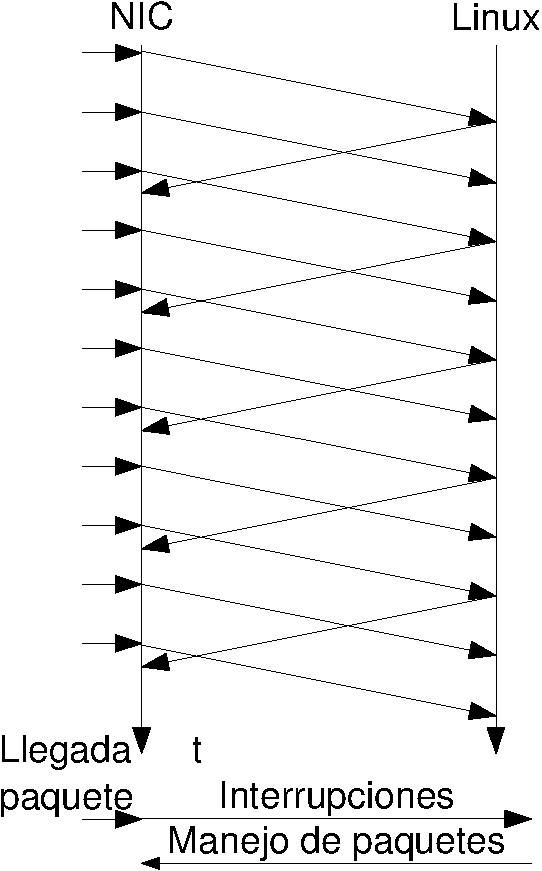
\includegraphics[width=0.30\textwidth]{CapituloPF_RING/Figuras/InterrupcionesNIC-crop}}%
\hspace{0.2\textwidth}
\subfloat[Device Polling]%
 {\LABFIG{DevicePolling}%
 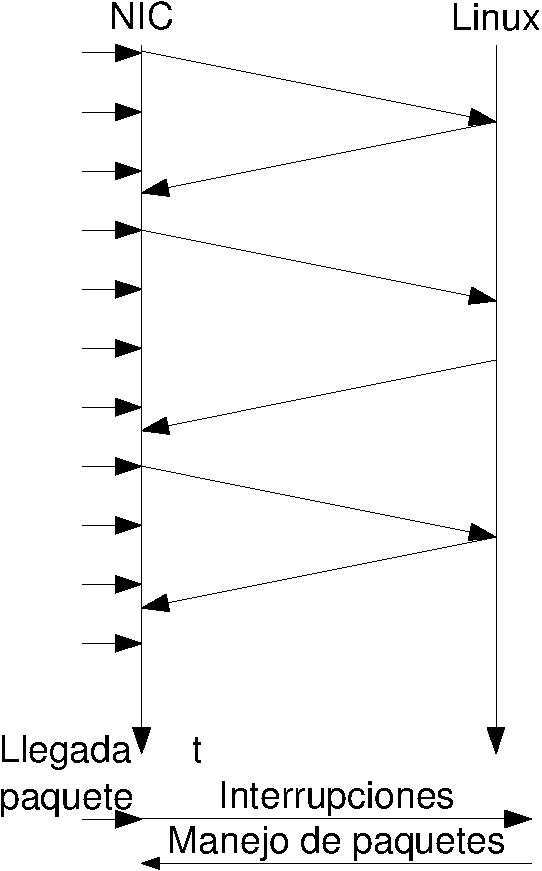
\includegraphics[width=0.30\textwidth]{CapituloPF_RING/Figuras/PollNIC-crop}}%
%
\caption{Comparativa entre los diferentes métodos de notificación de nuevos paquetes}
\end{figure}
%

\subsection{Obtención del paquete por parte del kernel}
Una interrupción debe ser rápida, esto es, en una interrupción no podemos realizar tareas que no sean estrictamente 
necesarias, por las mismas razones que las señales en espacio de usuario. Por ello, la interrupción provoca que se 
planee una tarea con el fin de recoger el paquete.

A partir de ese momento, sólo cuando el planeador decida que el sistema está libre, se recogerá el / los paquetes 
usando \texttt{packet\_rcv}, y se pasará a la pila de red de Linux.

En la pila, el paquete pasará por diversos sistemas, como la parte de filtrado 
\emph{\gls{netfilter}}\index{Netfilter} para, finalmente, ser recibido por un puerto o \emph{\gls{socket}} llegar a 
estar listo para la recogida por parte del espacio de usuario \cite{p206}.

\subsection{Obtención del paquete por parte del espacio de usuario}
La recepción de paquetes en el espacio de usuario se realiza mediante la librería \emph{\gls{libpcap}}\index{libpcap}.
Para ello, \emph{\gls{libpcap}} genera un \emph{\gls{socket}} que es abstraído por un descriptor de fichero. Si 
aplicamos la llamada al sistema \texttt{select} o \texttt{poll}, podemos saber si el socket dispone de datos para ser 
leídos, y leerlos en ese caso con la llamada \texttt{recvfrom}.

Un ejemplo de este tipo de lecturas podemos verlo en en \lstlistingname{}\ref{code:lecturaRawSocket}. En él, vemos la 
creación del socket con \texttt{socket}, la consulta de disponibilidad con \texttt{poll} y la recepción de los datos 
con \texttt{recvfrom}.

\begin{lstlisting}[language=C++,caption={Lectura desde un socket crudo}, 
breaklines=true, label=code:lecturaRawSocket,numbers=left,float=htbp]
#include<stdio.h>
#include<string.h>

#include<net/ethernet.h>
#include<sys/socket.h>
#include<arpa/inet.h>
#include<sys/ioctl.h>
#include<sys/types.h>
 
void ProcessPacket(char* , int);
 
int main(){
    size_t saddr_size, data_size;
    struct sockaddr saddr;
         
    char buffer[65536];
   
    int sock_raw = socket(AF_PACKET, SOCK_RAW, htons(ETH_P_ALL));
    setsockopt(sock_raw, SOL_SOCKET, SO_BINDTODEVICE, "eth0", 
                                               strlen("eth0")+1);
     
    if(sock_raw < 0){
        perror("Socket Error");
        return 1;
    }
    while(1){
        struct pollfd fds = { fd: sock_raw, events: POLLIN};
        const int poll_rc = poll(&fsd, 1, 1000);
        if(poll_rc == 0){
            if(poll_rc <= 0)
                perror("Poll error");
            continue;
        }
        saddr_size = sizeof(saddr);
        //Receive a packet
        data_size = recvfrom(sock_raw, buffer, 65536, 0, &saddr, 
                                       (socklen_t*)&saddr_size);
        if(data_size < 0){
            printf("Recvfrom error , failed to get packets\n");
            return 1;
        }
        //Now process the packet
        ProcessPacket(buffer , data_size);
    }
    close(sock_raw);
    return 0;
}
\end{lstlisting}

Sin embargo, este procedimiento tiene un coste oculto. A la hora de leer los datos, estos son copiados desde la 
memoria del núcleo a un buffer en espacio de usuario. Esto es, por cada paquete, estamos perdiendo tiempo y ciclos de 
CPU en copiar un dato que sólo vamos a leer.

Si, por ejemplo, queremos leer paquetes de 150kb en un enlace saturado a una velocidad de 1Gbps, estamos realizando:
\begin{itemize}
 \item $\frac{1G}{150k} \approx 7000$ llamadas al sistema con \texttt{poll} y otras tantas con \texttt{recvfrom}.
 \item Copiando entre regiones de memoria RAM a 1Gbps.
\end{itemize}

\section{La alternativa: PF\_RING}\LABSEC{La alternativa: PF RING}


\endinput

\begin{Resumen}[Resumen de PF RING]


\subsection*{S1}

\end{Resumen}


% 
%%:Empezamos con los apéndices, que irían en uno o más ficheros. Es necesario incluir estos ficheros entre el entorno \begin{appendices}....\end{appendices} debido a que se ha deseado utilizar un formato diferente para el título de los apéndices, incluyendo la palabra apéndice, para la numeración de los apéndices, alfabético, y para las cabeceras de las páginas.
%
%\begin{appendices}
%
%% Fichero en el que se incluyen los apéndices
%% !TEX root =../LibroTipoETSI.tex



%APENDICE A
\chapter{Sobre  \LaTeX}\LABAPEN{ApA}
{Este es un ejemplo de apéndices, el texto es únicamente relleno, para que el lector pueda observar cómo se utiliza}
%%%%%%%%%%%%%%%%%
\section{Ventajas de \LaTeX}

El gusto por el \LaTeX\ depende de la forma de trabajar de cada uno. La principal virtud es la facilidad de formatear cualquier texto y la robustez. Incluir títulos, referencias es inmediato.
%\Blindtext
%\lipsum
Las ecuaciones quedan estupendamente, como puede verse en \EQ{Ap1}
\begin{equation}\LABEQ{Ap1}
x_{1}=x_{2}.
\end{equation}


\section{Inconvenientes}
%\Blindtext
El principal inconveniente de \LaTeX\ radica en la necesidad de aprender un conjunto de comandos para generar los elementos que queremos. Cuando se está acostumbrado a un entorno ``como lo escribo se obtiene'', a veces resulta difícil dar el salto a ``ver'' que es lo que se va a obtener con un determinado comando. 

Por otro lado, en general será muy complicado cambiar el formato para desviarnos de la idea original de sus creadores. No es imposible, pero sí muy difícil. Por ejemplo, con la sentencia siguiente:
 
\begin{lstlisting}[language=,caption={Escritura de una ecuación}, breaklines=true, label=prgA1-01]
\begin{equation}\LABEQ{Ap2}
x_{1}=x_{2}
\end{equation}
\end{lstlisting}
obtenemos:
\begin{equation}\LABEQ{Ap2}
x_{1}=x_{2}
\end{equation}
Esto será siempre así. Aunque, tal vez, esto podría ser una ventaja y no un incoonveniente.

Para una discusión similar sobre el Word\tsp{\textregistered}, ver \APEN{ApB}.
%\Blindtext


%%%%%%%%%%%%%%%%%%%%%%%%%%%%%%%%%%%%%%%
%APENDICE B
\chapter{Sobre Microsoft Word\tsp{\textregistered}}\LABAPEN{ApB}

\section{Ventajas del Word\tsp{\textregistered}}
La ventaja mayor del Word\tsp{\textregistered} es que permite configurar el formato muy fácilmente. Para las ecuaciones,
\begin{equation}
x_{1}=x_{2},
\end{equation}
tradicionalmente ha proporcionado pésima presentación. Sin embargo, el software adicional Mathtype\tsp{\textregistered} solventó este problema, incluyendo una apariencia muy profesional y cuidada. Incluso permitía utilizar un estilo similar al \LaTeX\xspace. Además, aunque el Word\tsp{\textregistered} incluye sus propios atajos para escribir ecuaciones,  Mathtype\tsp{\textregistered} admite también escritura \LaTeX\xspace. En las últimas versiones de Word\tsp{\textregistered}, sin embargo, el formato de ecuaciones está muy cuidado, con un aspecto similar al de \LaTeX.


\section{Inconvenientes de Word\tsp{\textregistered}}
Trabajar con títulos, referencias cruzadas e índices es un engorro, por no decir nada sobre la creación de una tabla de contenidos. Resulta muy frecuente que alguna referencia quede pérdida o huérfana y aparezca un mensaje en negrita indicando que  no se encuentra. 

Los estilos permiten trabajar bien definiendo la apariencia, pero también puede desembocar en un descontrolado incremento de los mismos. Además, es muy probable que Word\tsp{\textregistered} se quede colgado, sobre todo al trabajar con copiar y pegar de otros textos y cuando se utilizan ficheros de gran extensión, como es el caso de un libro.

%\end{equation}
 %Ver este fichero para incluir ahí los apéndices.
%
%\end{appendices}
%:Fin de la inclusión de apéndices

%:Empieza todo lo que no constituye el cuerpo en si del libro. Todo lo que va detrás
\backmatter

%:Indice de figuras, coméntese las siguientes líneas si no se desea
\cleardoublepage
\phantomsection

%:Para añadir una línea en blanco en el TOC y separar esta lista
\addtocontents{toc}{\protect\mbox{}\protect\hspace*{0pt}\par}
\addcontentsline{toc}{listasb}{\listfigurename}
\pagestyle{especial}
\listoffigures

%:Indice de tablas, coméntese las siguientes líneas si no se desea
\cleardoublepage
\phantomsection
\addcontentsline{toc}{listasb}{\listtablename}
\pagestyle{especial}
\listoftables

%:Indice de Programas
\cleardoublepage
\phantomsection
\addcontentsline{toc}{listasb}{\lstlistlistingname}
\pagestyle{especial}
\lstlistoflistings

%:Bibliografía con biblatex y biber
\cleardoublepage
\phantomsection
\addcontentsline{toc}{listasb}{\bibname}
\pagestyle{especial}
%BIBER
%\printbibliography[heading=etsi]
%BIBTEX
%\bibliographystyle{IEEEtran}
\bibliographystyle{amsplain} %flexbib amsplain alpha
%:Fichero con la bibliografía, BIBTEX
\bibliography{bibliografiaLibroETSI}

%:Índice alfabético de palabras
\cleardoublepage
\phantomsection
\addcontentsline{toc}{listasb}{\indexname}
\chaptermark{\indexname}
\printindex


%:Acrónimos
\cleardoublepage
\phantomsection
\addcontentsline{toc}{listasb}{\glossaryname}
\chaptermark{\glossaryname}
\printglossaries

\end{document}